The experiments were done by considering two synthetic networks which consisted of $10^4$ and $10^5$ nodes. These two networks were generated using the same method used by the paper's authors, the Barabási-Albert model with preferential attachment, which enabled us to generate graphs which have similar properties as the social networks.

Each node contained only one random $(key, value)$ entry. In a real-world application, the $key$ should be a hash or a public key, here we simply generated a random number $k \in [0, 2^{31}-1]$ and a random IP address. 
Since $n \ll 2^{31}-1$ we assumed that all the elemenent generated were unique in the DHT.

In order to add Sybil nodes, we repeatedly chose a random node in the network and we turned it into a Sybil one. We kept converting nodes until we reached a number of attack edges equal to $g$.

Moreover, in order to simulate a clustering attack, we chose a random $key$ and we made all Sybil nodes to choose their layer-0 IDs such that: 
$\forall id \in ids(u, 0)$ where $u$ is Sybil, $id < key$. Ideally, Whanau do not embed a metric space into their keys, therefore, we artificially placed all the layer-0 Sybil's $id$s such that to make them ``close enough" to the target $key$.

We did several experiments in order to verify the most important assumption of Whanau: (1) \textbf{number of lookup messages decreases as the table size increases} (2) \textbf{clustering attacks only causes an increase of lookup messages} (3) \textbf{using layers makes Whanau resilient to clustering attacks} (4) \textbf{the number of lookup messages is constant if there is no attack}.

In order to have a statistically meaningful synthesis of the Whanau protocol behaviour, for each configuration (regarding network size, number of layers, etc.) we collected the statistics of 100 \textsc{lookup} calls (whether it failed or not and the number of messages sent around) in order to have a significant sample of data points.

\begin{figure}[t]
    \centering
    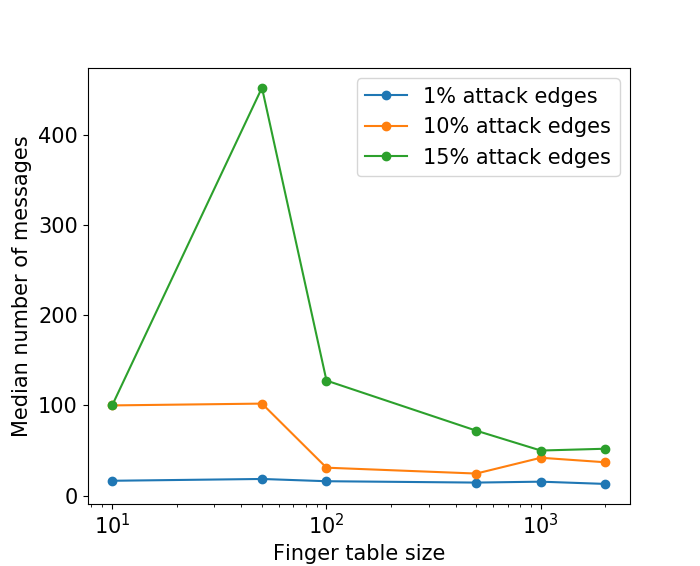
\includegraphics[scale=0.4]{exp1.png}
    \caption{Median number of messages delivered by \textsc{lookup} calls under different fingers table sizes. The performance were recorded also for different Sybil attack conditions ($\%$ of attack edges).}
    \label{fig:experiment_1}
\end{figure}

\subsection{\textsc{Lookup} calls vs. Routing rable size}

Figure \ref{fig:experiment_1} illustrates the behaviour of the protocol w.r.t. (1) finger table size (x-axis), (2) median number of messages (y-axis) and (3) percentage of attack edges.

As shown, as the finger table grows in size the number of messages tend to decrease: it's clearer in the examples with a higher percentage of attack nodes (10-15\%). The behaviour with 1\% of attack edges is basically identical to a network without malicious nodes, so it can be seen as a baseline performance for comparison purposes.
The collected datapoints are the different combinations of:
\begin{itemize}
    \item \textit{finger table size}: 10, 50, 100, 500, 1000, 2000
    \item \textit{attack edges \%}: 1\%, 10\%, 15\%
\end{itemize}
and \textit{network size} has been fixed to $10^4$. Moreover, we set to 3 the number of layers. Note that the \textit{x}-axis has a logarithmic scale.

These results confirm the simple intuition that if a node stores more known neighbours for each layer, it is easier to find the target key, avoiding all the Sybil nodes clustering. On the other hand, even though the fingers increase in an exponential fashion, having routing tables larger than a certain threshold do not bring much improvement to the performances w.r.t the number of messages.

\begin{figure}[t]
    \centering
    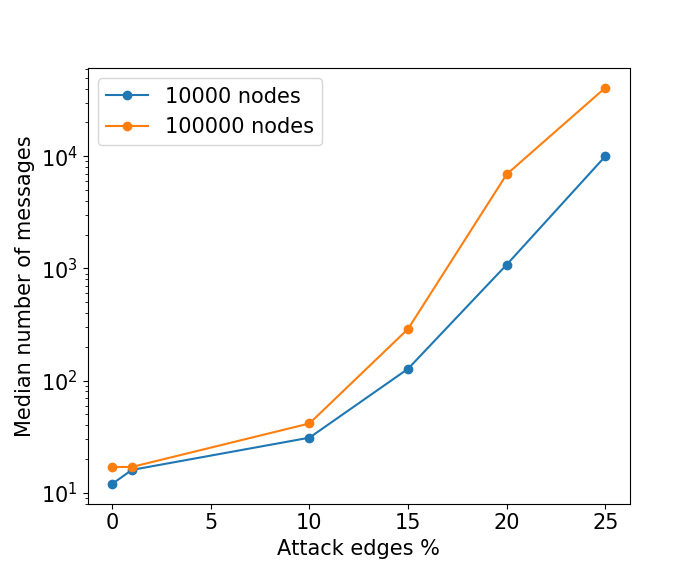
\includegraphics[scale=0.4]{exp2.png}
    \caption{Median number of messages sent by \textsc{lookup} node, given fixed layer and fixed routing tables size, by varying the percentage of attack edges.}
    \label{fig:experiment_2}
\end{figure}

\subsection{\textsc{Lookup} calls vs. Percentage of attack edges}

The second experiment aimed to study the response of the network under different increasing percentages of attack edges by using the default configurations parameter of Whanau.

We conducted two series of tests varying in the network size (respectively $10^4$ and $10^5$). The percentage of attack edges used were: 0\%, 10\%, 15\%, 20\%, 25\%. The number of layers is fixed to 3 and the fingers and successors tables were set to the theoretical defined size of  ($O(\sqrt{kn}) \approx 100$).

The paper specifies that the protocol has one-hop \textsc{lookup} performances when the number of attack edges is less than a predefined value $g \leq O(\frac{n}{w})$. 
Figure \ref{fig:experiment_2} shows that the median number of messages grows in the order of the thousands when the percentage of attack edges $g$ grows past the threshold the protocol allows to tolerate (e.g. \textit{g} should be in the order of the 10\% of the total nodes for $n=10^4$ ). It can be noticed that when $g\leq O(\frac{n}{w})$  the number of messages sent around is comparable to the case without attack edges.

\subsection{\textsc{Lookup} call is $O(1)$}

This experiment empirically shows how the protocol is a one-hop DHT in the absence of malicious identities. The number of layer of 3 and the fingers and successor tables are set as described above in the \textit{Experiment 2}.

The four test networks had respectively 5000, $10^4$, $10^5$ and $2\cdot 10^5$ nodes. The boxplots shown in Figure \ref{fig:experiment_3} shows that there are no particular differences regarding the number of messages sent for the different network sizes (despite having a different magnitude of nodes).

\subsection{Layers improve performances under clustering attacks.}

Figure \ref{fig:experiment_4} highlights the impact of having multiple layers when dealing with clustering attacks caused by Sybil nodes. The y-axis shows the percentage of the successful queries related to the percentage of edges that are compromised.

The protocol starts to suffer rapidly when there is just 1 layer and the percentage of attack edges grows out of the tolerable threshold of the system: around the 20\% mark, performances drops to 73\%. By using  3 or more layers, the protocol can cope with the difficulties imposed by the Sybil nodes, keeping the performance around 90\% of successful queries.

\begin{figure}[t]
    \centering
    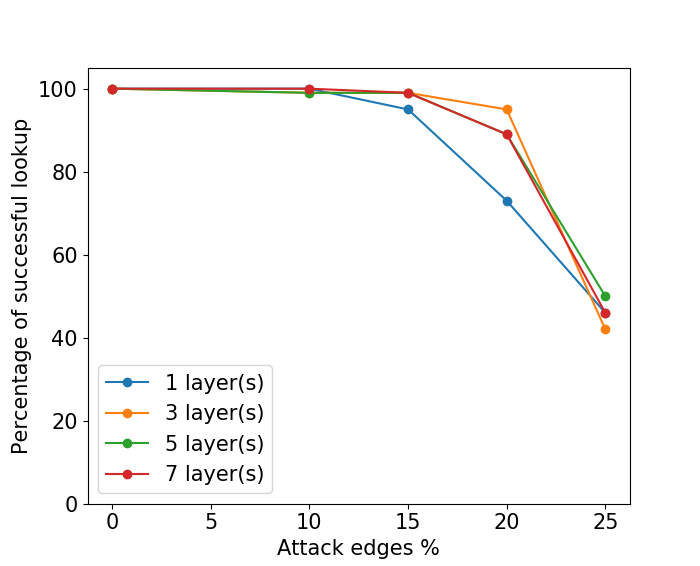
\includegraphics[scale=0.4]{exp4.png}
    \caption{Percentage of successful \textsc{lookup} calls under different percentages of attack edges. We tested several numbers of layers.}
    \label{fig:experiment_4}
\end{figure}